 % ==================================
% DO NOT EDIT
% ==================================
\documentclass[conference]{IEEEtran}
% *** CITATION PACKAGES ***
%
\ifCLASSOPTIONcompsoc
  % IEEE Computer Society needs nocompress option
  % requires cite.sty v4.0 or later (November 2003)
  \usepackage[nocompress]{cite}
\else
  % normal IEEE
  \usepackage{cite}
\fi
\usepackage{amsmath,amssymb,amsfonts}
\usepackage{algorithmic}
\usepackage{graphicx}
\usepackage{textcomp}
\usepackage{xcolor}
\usepackage{hyperref}
\usepackage{float}
\def\BibTeX{{\rm B\kern-.05em{\sc i\kern-.025em b}\kern-.08em
    T\kern-.1667em\lower.7ex\hbox{E}\kern-.125emX}}

\makeatletter
\newcommand{\linebreakand}{%
  \end{@IEEEauthorhalign}
  \hfill\mbox{}\par
  \mbox{}\hfill\begin{@IEEEauthorhalign}
}
\makeatother
% ==================================
% END
% ==================================


\begin{document}

\title{X-Care: A Suite of Rehabilitation Tools To Assist X-Ray Patients}

\author{

\IEEEauthorblockN{Dev Shah}
\IEEEauthorblockA{
    \textit{University of Waterloo} \\
    \href{mailto:d73shah@uwaterloo.ca}{d73shah@uwaterloo.ca}
}

\and

\IEEEauthorblockN{Hargun Mujral}
\IEEEauthorblockA{
    \textit{University of Waterloo} \\
    \href{mailto:hmujral@uwaterloo.ca}{hmujral@uwaterloo.ca}
}

\and

\IEEEauthorblockN{Ali Al-Hamadani}
\IEEEauthorblockA{
    \textit{University of Waterloo} \\
    \href{mailto:a2alhama@uwaterloo.ca}{a2alhama@uwaterloo.ca}   
}

\and
\IEEEauthorblockN{Helen Li}
\IEEEauthorblockA{
    \textit{University of Waterloo} \\
    \href{mailto:h273li@uwaterloo.ca}{h273li@uwaterloo.ca}
}

\linebreakand

% \and
\IEEEauthorblockN{Guruprasanna Suresh}
\IEEEauthorblockA{
    \textit{University of Waterloo} \\
    \href{mailto:grajukan@uwaterloo.ca}{grajukan@uwaterloo.ca}
}

\and
\IEEEauthorblockN{Mukund Chettiar}
\IEEEauthorblockA{
    \textit{University of Waterloo} \\
    \href{mailto:msayeega@uwaterloo.ca}{msayeega@uwaterloo.ca}
}

\and
\IEEEauthorblockN{Mica Shatil}
\IEEEauthorblockA{
    \textit{University of Waterloo} \\
    \href{mailto:mshatil@uwaterloo.ca}{mshatil@uwaterloo.ca}
}


% Uncomment below to add more authors

% \linebreakand 
% \IEEEauthorblockN{Guruprasana}
% \IEEEauthorblockA{
%     \textit{Queen's University} \\
%     email@email.com
% }
% 
% \and
% \IEEEauthorblockN{Full Name}
% \IEEEauthorblockA{
%     \textit{Queen's University} \\
%     email@email.com
% }
% 
% \and
% \IEEEauthorblockN{Full Name}
% \IEEEauthorblockA{
%     \textit{Queen's University} \\
%     email@email.com
% }


} % end authors

\maketitle


\begin{abstract}
This paper introduces a novel diagnostic tool that combines Supervised Learning in image classification, and Retrieval-Augmented Generation (RAG) using LLMs, to support the detection and diagnosis of injuries based on X-ray images for patients. By applying transfer learning with specialized datasets on DenseNet and EfficientNet convolutional neural networks (CNNs), which were pretrained on the ImageNet dataset, the tool approaches expert-level accuracy in detecting and classifying various skeletal fractures. Then, the RAG-powered rehabilitation agent allows for informative plans and recommendations, using clinically verified documents from a comprehensive medical database (PubMed). The fusion of these technologies offers significant potential to improve patient care by providing rapid and sophisticated analyses, in an effort to bridge the gap between diagnostic imaging and consultation with a professional to enable a quicker recovery and reduce patient uncertainty. 
\end{abstract}

\section{Introduction}

There is an urgent necessity to advance the quality and speed of X-ray diagnosis. As it currently stands, there is an average delay of 14-days\cite{VCH} between performing an X-ray scan and an appointment with a specialist to discuss results. This gap not only hinders the diagnostic process but also leaves patients in a state of uncertainty and anxiety while awaiting further consultation with healthcare specialists. And considering that up to 25\% of X-rays are rejected or must be repeated \cite{BMC2017}, this issue is exacerbated. Thus we hope to tackle the  problem of the absence of immediate rehabilitative guidance for patients throughout prevalent X-ray procedures. 

\subsection{Motivation}


Conventional methods of interpreting X-ray images are often hampered by speed and variability of human analysis, which can yield inconsistent diagnostic outcomes \cite{Kuo2022AI}. By employing Supervised Learning and Retrieval-Augmented Generation (RAG), we strive for diagnostic precision and consistency surpassing traditional human-led evaluations.

Our aspirations, however, extend beyond diagnostics. Leveraging AI to scrutinize X-ray data, we aim to offer patients personalized rehabilitation plans and provide immediate, informed responses to their queries. This approach is designed to kickstart recovery ahead of specialist consultations, providing vital, timely advice when it is most needed \cite{Sharma2023}.

The fundamental objective is to elevate patient outcomes through rapid, precise diagnostics and early intervention strategies. Through this project, we underscore our commitment to the application of state-of-the-art AI technologies within the healthcare field, contributing to diagnosis and facilitating a seamless recovery journey. 






% Our project addresses the critical need for enhancing medical diagnostics and patient support using AI technologies, including Computer Vision and Retrieval-Augmented Generation (RAG). Traditional X-ray analysis methods, limited by speed and variability in human judgment, often lead to inconsistent diagnoses \cite{Kuo2022AI}.  By employing AI, we aim for consistent, accurate evaluations that exceed human analysis capabilities.


% Moreover, our initiative expands beyond diagnostics. Upon analyzing X-rays with AI, we will offer patients personalized rehabilitation plans and answer their immediate questions. This proactive approach aims to kick start the healing process ahead of specialist consultations, providing essential guidance during the interim \cite{Sharma2023}.

% Our overarching goal is to improve patient outcomes through rapid, precise diagnostics and early intervention strategies. This project signifies our commitment to integrating advanced technology with healthcare, ensuring AI's role extends from diagnostics to facilitating a seamless recovery journey.

\section{Related Work}

Multiple studies have highlighted the efficacy of artificial intelligence in the realm of radiography-based fracture detection. A comprehensive review by a team of researchers in England, encompassing 42 studies, revealed comparable diagnostic performance between AI and clinicians, with both exhibiting a sensitivity of 91-92\% \cite{Kuo2022AI}. Notably, the BoneView model released by startup Gleamer in France, demonstrated proficiency to a degree higher than musculoskeletal radiologists in detecting fractures across diverse anatomical regions \cite{BoneView}. Their approach reduced missed fractures by 29\% and enhanced sensitivity by 16\%, illustrating the promise of AI in the field of orthopaedic radiology \cite{Guermazi2022AI}.

Presently, the most common methodology involves training AI models using deep learning networks. A study demonstrated the effectiveness of re-training a pre-existing CNN model, specifically an Inception v3 model, which achieved a binary classification model with 90\% sensitivity and 88\% specificity in fracture detection \cite{KIM2018439}. Additionally, a group of doctors and researchers from Sweden utilized openly available deep learning networks to create AI fracture detectors that performed similarly to senior orthopaedic surgeons when analyzing medical images \cite{Olczak2017AIOrtho}.

Although numerous works have shown the effectiveness of employing pre-trained deep-learning networks for the task of classifying fractures, integrating AI into real-world systems to benefit patients beyond mere fracture detection persists to be an issue. Novel techniques using Large Language Models (LLMs), such as RAG, have proven to reduce hallucination and provide accurate information when summarizing radiology papers, extracting relevant information and returning deterministic data \cite{lewis2021retrievalaugmented}. This approach can provide patients with recent and precise information extending from the training data in the LLM, and when used effectively toward creating rehabilitation plans, can allow for the initiation of treatment without delays \cite{Sharma2023}.


\section{Methodology}
\subsection{X-Ray Classification \& Recognition: Approach}
Our methodology for X-ray image recognition and interpretation would be divided into two phases: binary classification to determine the exstence of a fracture, and the subsequent identification of the fracture's precise location within the X-ray scan. 

\paragraph{Initial Research and Planning}
We commenced the project with an in-depth investigation into the prevalent challenges within X-ray dagnostics, followed by strategic planning. For the binary classification task, we selected to experiment between DenseNet and EfficientNet architectures, targeting the detection of fractures with the FracAtlas Dataset. For localization of fractures, we 
planned to incorporate an object detection model, such as Faster R-CNN.
% The initial stage involved researching the problems and devising a plan. We opted to use a DenseNet model for binary classification, with the aim of identifying the presence or absence of a fracture using the FracAtlas Dataset. An object detection algorithm, such as Faster R-CNN, was incorporated for detecting the fracture's location.

\paragraph{Revised Approach}

During the exection phase, we encountered hurdles with the quality of our R-CNN model and the practicality of integrating an object-detection approach with our planned workflow. Theses challenges necessitated a revised approach, leading to the decision of building two CNN-based classification models to independently handle each phase: A binary classifier for fractures, and a multiary classificatier for localization. For the latter, this also required searching for a new dataset more comprehensive in body part classification.
% Upon implementation, we faced challenges integrating Faster R-CNN with DenseNet and discovered limitations in the FracAtlas dataset. Consequently, we adjusted our strategy to assign dedicated models for each step and sought a new dataset for more comprehensive body part classification.
\subsection{Step 1: Presence of a Fracture}
\subsubsection{Model Information}
To train our fracture detection model, we utilized the FracAtlas dataset \cite{FracAtlas}, comprising 4,083 annotated X-ray images. Using the DenseNet121 and EfficientNet architectures as backbones, and weights from pre-trained artifacts using the ImageNet dataset, we trained the models to classify X-ray images as either fractured (1) or non-fractured (0). We used a 70:15:15 split for training, testing and validation to ensure the model's generalization.

% We utilized  DenseNet architecture for its efficiency in feature extraction, crucial for the binary classification task at hand. The classification was binary, with labels 1 (fractured) and 0 (not fractured). The dataset was divided into training, validation, and testing sets with a ratio of 70:15:15, ensuring a balanced approach to model training and evaluation.



\subsubsection{Testing Results}
We iterated on testing different hyperparameters and configurations to optimize the model's performance. By using Optuna, a hyperparameter optimization framework, we employed the Tree-structured Parzen Estimation algorithm to search for the best hyperparameters. This approach of Bayesian optimization allowed us to fine-tune the model's hyperparameters, including the number of epochs, batch size, optimizer, and learning rate.

The initial reference models' hyperparameters, configurations, and accuracy are located in Table~\ref{table:comparison1} and Table~\ref{table:comparison2}.

\begin{table}[H] % Forces the table to be placed here in the document
\centering
\caption{Comparison of Model Parameters and Performance Before and After Tuning (EfficientNet)}
\label{table:comparison1}
\begin{tabular}{|l|c|c|}
\hline
\multicolumn{1}{|c|}{\textbf{Parameter}} & \textbf{Initial} & \textbf{Tuned} \\ \hline
\#(Epochs)                               & 5                & 3              \\ \hline
Batch Size                               & 64               & 64             \\ \hline
Loss Function                            & BCE              & BCE            \\ \hline
Optimizer                                & SGD              & Adam           \\ \hline
Learning Rate                            & 0.001            & 0.001          \\ \hline
Validation Accuracy                      & 74.56\%          & 88.40\%        \\ \hline
Test Accuracy                            & 71.84\%          & 86.60\%        \\ \hline
\end{tabular}
\footnotesize
\end{table}
\begin{table}[H] % Forces the table to be placed here in the document
\centering
\caption{Comparison of Model Parameters and Performance Before and After Tuning (DenseNet)}
\label{table:comparison2}
\begin{tabular}{|l|c|c|}
\hline
\multicolumn{1}{|c|}{\textbf{Parameter}} & \textbf{Initial} & \textbf{Tuned} \\ \hline
\#(Epochs)                               & 5                & 2              \\ \hline
Batch Size                               & 64               & 32             \\ \hline
Loss Function                            & BCE              & BCE            \\ \hline
Optimizer                                & SGD              & Adam           \\ \hline
Learning Rate                            & 0.001            & 0.00019          \\ \hline
Validation Accuracy                      & 73.69\%          & 86.30\%        \\ \hline
Test Accuracy                            & 70.65\%          & 85.15\%        \\ \hline
\end{tabular}
\footnotesize
\begin{flushleft}
BCE: Binary Cross Entropy Loss.
\end{flushleft}
\end{table}

We had inferred from manual inspection of the various trials with different hyperparameter configurations that 3 epochs were sufficient for the model to converge, and
more epochs did not significantly impact the test accuracy. After fine-tuning the hyperparameters, we achieved a validation accuracy of 86.6\% with the EfficientNet model, a significant improvement over the initial 71.84\% accuracy.

Upon experimentation, we saw that, almost universally with the same hyperparameter configurations, EfficientNet outperformed DenseNet in terms of accuracy. Thus, we opted to allocate more resources to testing and tuning the EfficientNet model. 


\subsection{Step 2: Fracture Location (Multiary Classification)}
In this step, we focus on the body part classification of detected fractures based on their location within X-ray images. Identifying a suitable dataset for this purpose required a comprehensive review of available resources, as many lacked specificity and comprehensive labelling. Below, we detail our evaluation of several datasets considered for this task.

% \subsubsection{Datasets for Multi-class Classification}
% Our search for appropriate datasets yielded three promising candidates, each with distinct features and potential applications in fracture location classification.

\paragraph{UNIFESP X-Ray Body Part Classification Dataset}
This dataset consists of 2,481 X-ray images across 22 body parts, annotated in a multilabel format, making it ideal for detailed classification tasks in our second step.

\paragraph{VinDr-BodyPartXR}
Derived from DICOM scans, it includes general labels such as "abdominal," "pediatric," and "adult." Its broad categorizations, however, lacked the specificity needed for precise classification in our study.

\paragraph{MURA (Musculoskeletal Radiographs)}
A large collection focusing on upper body parts, including 7 specific areas. While extensive, its scope was too narrow for the broad classification goals of our project.\\


We thus selected the UNIFESP dataset for its comprehensive coverage of body parts, which aligned with our classification objectives. 

\subsubsection{Model Information}
We built off of a DenseNet architecture, and tailored it's output layer to support 22 output classes. The training and testing were conducted on an 80:20 split.

\subsubsection{Data Preprocessing}
Upon examination, it was discovered that only the published training set of the UNIFESP dataset had labels. Thus, the number of usable images dropped to 1738 images. Additionally, some images in the dataset were labelled with multiple body parts, which were removed to simplify the classification task and remove unnecessary complexity. This resulted in a final dataset of 1606 images.

The data labels, represented as numerical values ranging from 0 to 21 for each body part, and a 80:20 ratio was employed ratio for training and testing respectively. Due to the small size of the dataset, we wanted to include as many images as possible in the training set, and thus did not use a test set.
 We intend on experimenting with data augmentation techniques to artificially increase the size of the dataset in the future.

\subsubsection{Testing Results}
In the initial trial, the model was trained with configurations summarized in Table~\ref{tab:model_performance}. 

\begin{table}[H]
\centering
\caption{Model Configuration and Performance}
\label{tab:model_performance}
\begin{tabular}{|l|c|c|}
\hline
\textbf{Parameter} & \textbf{Initial} & \textbf{Tuned} \\ \hline
\#(Epochs) & 9 & 5 \\ \hline
Batch Size & 64 & 32 \\ \hline
Optimizer & SGD & Adam \\ \hline
Learning Rate & 0.001 & 0.0001 \\ \hline
Validation Accuracy & 96.18\% & 99.38\% \\ \hline
Test Accuracy & 90.06\% & 91.30\% \\ \hline
\end{tabular}
\end{table}

As shown, the validation accuracy was exceptionally high, reaching up to 99.38\%. This hints at a high likelihood of overfitting, and further investigation is required to ensure the model's generalizability. 
Notably, the final test accuracy was 91.30\%, which is higher than expected and a potential cause for concern, considering the task of classifying between 22 labels. 

In an attempt to tackle this overfitting, we programmatically checked for image duplicates. Although all images were unique, many shared similarities in terms of backgrounds and bone placement. This lead to data invariance, and potentially contributed to the overfitting. 
Consequently, we concluded that training the model with a reduced number of epochs (3-5) would be more appropriate, however this needs to be revisited in the future.


Next, ten different model configurations with 3-5 epochs were tested, and the highest scoring model was selected as the final "tuned" result.
We employed manual hyperparameter tuning for this task, by running multiple trials with different configurations in parallel, and iteratively adjusting the hyperparameters based on the results of the trials. 

Among the ten models, three exhibited high accuracy ($>70\%$), while the remaining models yielded accuracy below 50\%. This hinted at very high variance, potentially related to the earlier issues of overfitting. To ensure consistent weight initialization across all models, the top-performing models were assessed with a fixed seed.

In general, regarding our specific task, the batch size seemed the least relevant, as successful models were achieved with varying batch sizes. Optimizers SGD and Adam performed well, alongside effective learning rates of 0.001 and 0.0001, as well as weight decays of 0.001 and 0.1.

Further investigation showed that a learning rate of 0.01 would adversely affect the highest accuracy model, and Adam remains the ideal optimizer for this task.

\subsubsection{Exploratory Advances in Fracture Detection - Employing Faster R-CNN}

This research employs a Faster R-CNN model with a ResNet50 backbone, renowned for its object detection prowess, to pinpoint fractures in medical imaging data from the FracAtlas dataset. The methodology integrates data pre-processing, such as image resizing and normalization, and leverages transfer learning to utilize pre-trained weights, enhancing the model’s capability to detect fractures accurately \cite{Ren2015FasterRT}. Hyperparameter optimization is performed using Optuna, focusing on learning rate, weight decay, and the number of epochs to refine model performance. The training process involves batch processing, forward and backward passes, and loss computation, with the Stochastic Gradient Descent (SGD) optimizer chosen for its effectiveness in deep learning model training. The model is periodically evaluated on a validation set to monitor performance and adjust hyperparameters accordingly \cite{TorchvisionFasterRCNN}.

\begin{table}[H]
\centering
\caption{Performance Metrics of Model Training Across Different Hyperparameters}
\label{tab:model_hyperparameters}
\begin{tabular}{|l|c|c|c|c|}
\hline
\textbf{S.No} & \textbf{Mean IOU} & \textbf{Lr} & \textbf{Weight\_decay} & \textbf{No of epochs} \\ \hline
1 & 0.2032 & 0.00082 & 0.00011 & 6 \\ \hline
2 & 0.2270 & 0.00095 & 0.00011 & 5 \\ \hline
3 & 0.2177 & 0.00091 & 0.00010 & 5 \\ \hline
4 & 0.2033 & 0.00044 & 0.00042 & 5 \\ \hline
5 & 0.2470 & 0.00098 & 0.00022 & 5 \\ \hline
6 & 0.2175 & 0.00032 & 0.00037 & 6 \\ \hline
\end{tabular}
\end{table}


The table ~\ref{tab:model_hyperparameters} lists the outcomes of multiple runs with varying hyper parameters. The `Mean\_IOU` column represents the mean Intersection over Union, a common metric for evaluating the accuracy of an object detector on a particular dataset. The `Lr` column indicates the learning rate, `Weight\_decay` is a regularization term to prevent over fitting, and `No of epochs` shows how many complete passes the algorithm has made over the entire training dataset.

\textbf{Results:} The dataset records indicate that the model performed best with a mean IOU of approximately 0.2471 when the learning rate was set to roughly 0.000988, paired with a weight decay of about 0.000225 over the course of 5 epochs. Notably, this configuration achieved the highest recorded mean IOU without the need for the most extended training period, indicating a more efficient learning process compared to other configurations. In contrast, the lowest mean IOU observed was approximately 0.2033 with a significantly lower learning rate of 0.000442 and a higher weight decay of 0.000420 across 5 epochs. This outcome could suggest that either the learning rate was too low for the model to make significant updates to its weights or the high weight decay overly penalized the model parameters, hindering its ability to fit the data effectively.
In general, for our specific task, the batch size was least relevant, as successful models were achieved with varying batch sizes. Optimizers SGD and Adam both performed well, alongside effective learning rates of 0.001 and 0.0001 and weight decays of 0.001 and 0.1.

\subsection{Patient Diagnosis: RAG}
To generate an accurate diagnosis for the provided X-ray, we build a customized Retrieval Augmented Generation (RAG) pipeline. This pipeline retreives document chunks sourced from the PubMed database of clinically verified medical documents, using their querying tool to find papers and journals related to X-ray imaging and rehabilitation. 

We integrated two textual embedding models for similarity search: `all-MiniLM-L6-v2', an open-source model hosted on HuggingFace, and OpenAI’s `text-embedding-002-ada' model. We also added support and tooling for two Large Language Models (LLMs): Cohere's `Command Nightly', and OpenAI's `GPT-4-Turbo'. We generalized our modules in a way that we can support the integration of new models easily. 

% These models were selected to balance cost and performance, with the HuggingFace model serving as a cost-effective alternative to the more expensive OpenAI model. Additionally, the pipeline utilizes two Large Language Models (LLMs): Cohere’s prompting LLM and OpenAI’s GPT-4, providing alternatives for cost efficiency and accuracy.

We elected to use RAG over fine-tuning an LLM, as the former has demonstrated accuracy with smaller datasets \cite{lewis2021retrievalaugmented}, is prone to hallucination and innacurate information, and it is impractical to annotate each prompt for fine-tuning. 

% The RAG approach was preferred over fine-tuning models like GPT-4 due to its demonstrated accuracy with smaller datasets and the impracticality of annotating each prompt for GPT-4 fine-tuning. In the pre-processing stage, medical diagnosis documents from PubMed and Springer were converted into vector embeddings using Cohere’s Embedding model.

Upon the system's ingestion and processing of a user's X-ray, information about their diagnosis is used to query a ChromaDB Vector Database instance. Relevant documents are then retrieved to provide context for the LLM, generating a natural language diagnosis response. 

% The system ingests and processes X-ray images, pinpointing fracture locations alongside patient data to search a vector database, retrieving pertinent information to aid GPT-4's diagnostic response.

% Initially, the most valuable medical documents for accurate diagnoses were gathered from Pubmed and Springer, chosen for their extensive, high-quality databases. Pubmed was favored for its straightforward API, and Springer's content was extracted via web scraping.

% For efficient RAG system operation, documents were broken down into uniform 100-character chunks. This size was optimal for maintaining context and ensuring consistent, effective embedding for better database searches.

% The chunked documents are then embedded, using either HuggingFace or higher-dimension OpenAI embeddings via Langchain, and stored with metadata in a Chroma database.

% In use, a user's query is vectorized and matched against the document chunks in Chroma. The top five relevant pieces form the basis of the LLM response—enriched by both Cohere and GPT-4 models—providing an informed reply grounded in the specific facts from the documents. The user receives this alongside source citations, ensuring transparency and veracity.



% Upon classification of the user’s X-Ray image and embedding of the fracture location and other patient information, this data is used to query a vector database. Relevant documents are then retrieved to provide context for the GPT-4 LLM, which generates the diagnosis response.
% \subsubsection
The first stage in building the RAG system was to identify high value medical diagnosis documents that can be considered factual information. After reviewing over ten sources of medical research papers, Pubmed and Springer were decided as the top two sources due to the quality, scope, and size of their databases. Furthermore, Pubmed's API enables easy data ingestion. In Springer's case, beautiful soup was used to scrape the articles.

The second step of implementing the RAG pipeline is to chunk these documents. We explored chunking at a paragraph and sentence level before finally settling on a 100 character chunk size. Paragraphs vary too much in size making it difficult to properly embed each paragraph, and sentences often did not contain enough context. using a 100 character chunk size we found that the chunks have adequate context, and being a consistent size allows for better embedding of the chunks, and thus improved search for relevant documents.

Once the documents are chunked they are embedded using HuggingFace or OpenAI embeddings, both utilized from the Langchain Python interface. HuggingFace embeddings are free, but OpenAI's embeddings are of a much higher dimension by default, enabling more refined search. Each chunk of the documents is then embedded and stored with some metadata in a Chroma database. 

The chunks are stored in a Chroma DB ...

Now that all of the data has been ingested, we can utilize these documents in our RAG flow. When a user sends a query, their query is embedded into the same vector space the Chroma-db is in. A similarity search is run in Chroma between the document chunks and the query to return the top 5 most relevant document chunks to the query. We take these 5 most similar chunks and send them as RAG documents to the llm model when we submit the user query. Both Cohere’s prompting LLM and OpenAI’s GPT-4 llm take the similar chunks as document parameters and use them to form a response to the query using not only their general knowledge, but also the specific fact based information in the document chunks. Cohere’s prompting LLM is used from Cohere's python interface, and OpenAI’s GPT-4 is used from the Langchain interface. The llm's process the query and RAG documents, creating a response that is informed on related and factual medical information from the RAG documents. The response is sent back to the user along with document metadata to provide a legitimate citation for the sources of medical information. 

For a visual representation of this flow see Fig. 1. RAG Pipeline.

\begin{figure}
\centering
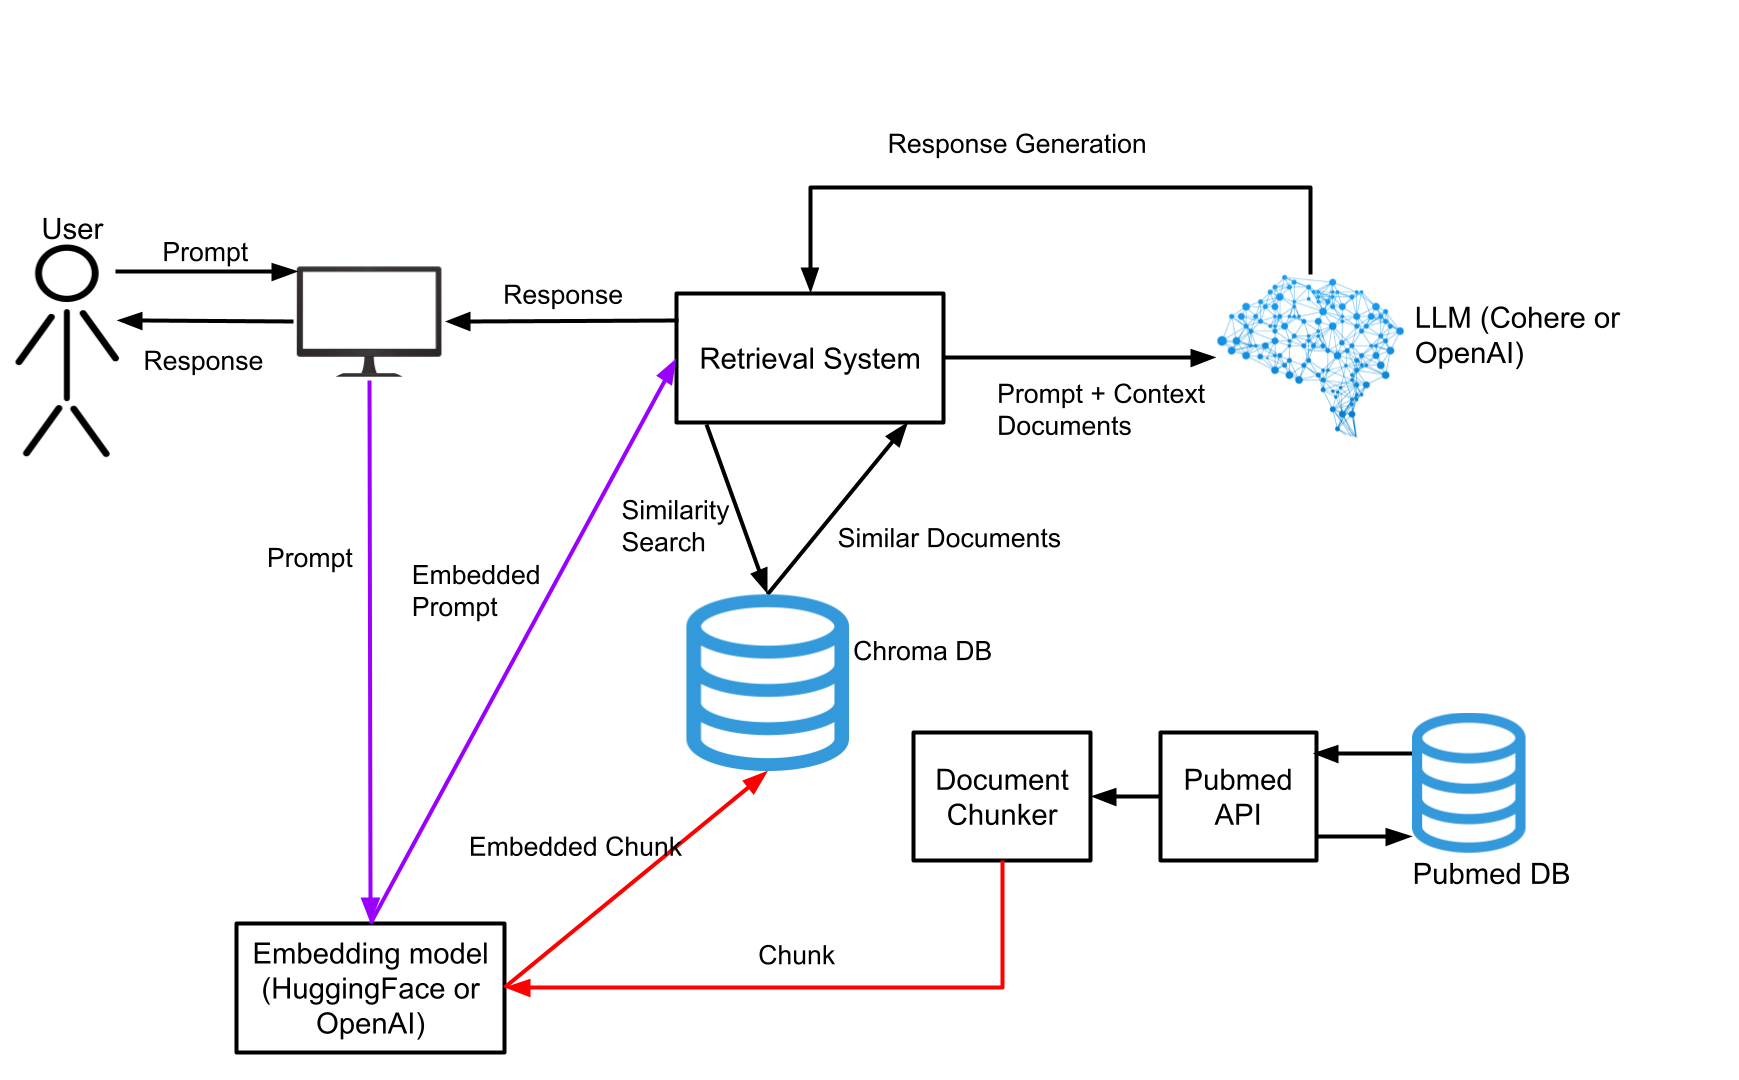
\includegraphics[width=\columnwidth]{RAG_flow.png}
\caption{RAG Pipeline}
\label{fig:image1}
\end{figure} 

\subsection{Proof Of Concept: Deliverable Application Interface}
We created a full-stack application using a React.js frontend, a FastAPI backend and cloud server hosting, to create both an application and user interface to communicate with the Machine Learning models. The 'X-Care' application 
supports users through two steps that interact with the technologies we researched and developed in this paper. 
\subsubsection{Fracture Identification and localization}
The user uploads their X-ray image, which is then analyzed by the two CNNs. The former first detects the presence of a fracture, and depending on the outcome, the system either stops with a notification of no issues, or proceeds to run inference on the second CNN to localize the injury.
After identifying both items, the user may override or correct the results as necessary.

\subsubsection{Diagnosis and Treatment Suggestions}
Next, users receive a diagnosis summary and a suggested treatment plan, generated by the 'User Flows' as described in the previous section. They have the option to modify and refine their treatment plan through certain user inputs in the interface, and interact with a general chat agent
powered by the RAG pipeline to ask specific questions about their injury and receive more information.

A link to the GitHub repository can be found here: \href{https://github.com/WAT-ai/X-Ray-Tooling}{https://github.com/WAT-ai/X-Ray-Tooling}.


\section{Conclusion}
The waiting period that exists between having diagnostic imaging taken and consultation with a doctor can be bridged, providing better patient care, speeding up recovery and reducing the period of uncertainty that follows injuries. The utilization of Supervised Learning and Retrieval Augmented Generation to create a diagnostic tool that improves accuracy and efficiency of X-ray fracture diagnosis can be achieved, as shown in the preceeding sections. We attempted employing a Faster RCNN model with a ResNet50 backbone, which resulted in low accuracy, making it impractical for application during  the current stage of the product. However, we achieved high functional accuracies utilizing CNN's trained on an extensive dataset while leveraging DenseNet and EfficientNet models. Overfitting issues were identified within the X-Ray localization model, which will be improved in future iterations. Quick, accurate and medically relevant information was successfully delivered to users, through the usage of a RAG pipeline that retrieved relevant data from a PubMed document database. Impactful outcomes for reduction of waiting times for consultations regarding results and follow-up procedures are clearly observed. 

\subsection{Results}
Our results demonstrate that our initial goal of producing a pipeline capable of diagnosing a fracture given an X-ray was successful. For Step 1 \& 2 (identifying the presence of a fracture and classifying a fracture's location), the DenseNet and EfficientNet models demonstrated high-quality results: following training and hyperparameter tuning, the models were able to achieve an accuracy of 86.60\% and 91.30\% respectively on an unseen 'test' dataset. 

\subsection{Future Work}
Looking ahead, our focus will be on improving our machine learning models and user-facing website for practical application in healthcare. This will entail engaging with clinicians in real hospitals, and medical researchers at Universities to deeply understand their needs and how our product can be best integrated into clinical workflows. We aim to refine our model's accuracy and architecture through rigorous testing and iterative development. Simultaneously, we plan to broaden our portfolio of tools, ensuring a comprehensive suite that addresses a wide range of medical needs.

% \section{Results}
% Our results demonstrate that our initial goal of producing a pipeline capable of diagnosing a fracture given an X-ray was successful. For Step 1 \& 2 (identifying the presence of a fracture and classifying a fracture's location), the DenseNet and EfficientNet models demonstrated high-quality results: following training and hyperparameter tuning, the models were able to achieve an accuracy of 86.60\% and 91.30\% respectively on an unseen 'test' dataset. 

% % \subsection{Replication Package}
% % If you have a public github or Kaggle Notebooks that people can run to replicate your experiments, uncomment and link them here like this: ~\href{https://www.kaggle.com/code/rababazeem/aeslc-kcentergreedy/notebook?scriptVersionId=158372243}{AESLC Kaggle Notebook}. 

% \section{Conclusion}
% Having introduced a diagnostic tool that integrates Computer Vision and RAG AI, this product significantly improves the accuracy and efficiency of X-ray image diagnosis in the medical field. Leveraging DenseNet and EfficientNet CNNs trained on extensive datasets, the Computer Vision models achieved high functional accuracies. The RAG element ensures that users receive the most accurate and scientifically valid information by retrieving relevant data from the PubMed papers database. Delivering quick, accurate, and up-to-date information through an electronic matter generates impactful outcomes for patient care, including the elimination of extended waiting times for doctor consultations regarding results and follow-up procedures.

% \section{Future Work}
% Looking ahead, our focus will be on improving our machine learning models and user-facing website for practical application in healthcare. This will entail engaging with clinicians in real hospitals, and medical researchers at Universities to deeply understand their needs and how our product can be best integrated into clinical workflows. We aim to refine our model's accuracy and architecture through rigorous testing and iterative development. Simultaneously, we plan to broaden our portfolio of tools, ensuring a comprehensive suite that addresses a wide range of medical needs.







% \section{Limitations}
% Talk about any limitations you experienced during your project here related to resources, time, or any other constraints.

% \section{Acknowledgements}
% If any individuals or organizations helped you with your project or your paper, make sure you acknowledge them here.

% \newpage

% \section{Appendix}
% Use this section to add additional figures and tables.

%% The next two lines define the bibliography style to be used, and
%% the bibliography file.
\bibliographystyle{apalike}
\bibliography{references}

\end{document}